\documentclass[preprint,12pt]{elsarticle}
\usepackage{amsmath}
\usepackage{latexsym}
\usepackage{graphicx}
\usepackage{xspace}
\usepackage{color}
\usepackage{array}
\usepackage{multirow}
\usepackage{hyperref}
\usepackage{wasysym}
\usepackage{verbatim}
\usepackage[font=normalsize]{caption}
\usepackage{mathtools}
\usepackage{relsize}
\addtolength{\oddsidemargin}{-.875in}
\addtolength{\evensidemargin}{-.875in}
\addtolength{\textwidth}{1.75in}
%\addtolength{\voffset}{-70pt}
%\addtolength{\textheight} {120pt}

\newcommand{\Otwo}{\ensuremath{\rm O_2}\xspace}
\newcommand{\Ntwo}{\ensuremath{\rm N_2}\xspace}
\newcommand{\CHfour}{\ensuremath{\rm CH_4}\xspace}
\newcommand{\Argon}{argon\xspace}
\newcommand{\Ar}{\ensuremath{\rm Ar}\xspace}
\newcommand{\ArR}{\ensuremath{\rm ^{39}Ar}\xspace}
\newcommand{\Kr}{\ensuremath{\rm Kr}\xspace}
\newcommand{\KrR}{\ensuremath{\rm ^{85}Kr}\xspace}
\newcommand{\meth}{methane\xspace}
\newcommand{\He}{\ensuremath{\rm He}\xspace}
\newcommand{\water}{\ensuremath{\rm H_2O}\xspace}
\newcommand{\AMU}{\ensuremath{\rm u}\xspace}
 
\newcommand{\ppm}{\ensuremath{\rm \cdot10^{-6}~g/g}\xspace}
\newcommand{\oneppm}{\ensuremath{\rm 10^{-6}~g/g}\xspace}
\newcommand{\ppb}{\ensuremath{\rm \cdot10^{-9}~g/g}\xspace}
\newcommand{\oneppb}{\ensuremath{\rm 10^{-9}~g/g}\xspace}
\newcommand{\ppt}{\ensuremath{\rm \cdot10^{-12}~g/g}\xspace}
\newcommand{\oneppt}{\ensuremath{\rm 10^{-12}~g/g}\xspace}
\newcommand{\nbb}{\ensuremath{\beta\beta 0\nu}\xspace}
\newcommand{\tbb}{\ensuremath{\beta\beta 2\nu}\xspace}
\newcommand{\xe}{\ensuremath{\rm xenon}\xspace}
\newcommand{\Xe}{\ensuremath{\rm xenon}\xspace}
\newcommand{\K}[1]{\ensuremath{\rm ^{#1}K}\xspace}
\newcommand{\U}[1]{\ensuremath{\rm ^{#1}U}\xspace}
\newcommand{\Th}[1]{\ensuremath{\rm ^{#1}Th}\xspace}
\newcommand{\Pb}[1]{\ensuremath{\rm ^{#1}Pb}\xspace}
\newcommand{\Po}[1]{\ensuremath{\rm ^{#1}Po}\xspace}
\newcommand{\Tl}[1]{\ensuremath{\rm ^{#1}Tl}\xspace}
\newcommand{\Ac}[1]{\ensuremath{\rm ^{#1}Ac}\xspace}
\newcommand{\Bi}[1]{\ensuremath{\rm ^{#1}Bi}\xspace}
\newcommand{\Cs}[1]{\ensuremath{\rm ^{#1}Cs}\xspace}
\newcommand{\KTHU}{K, Th, and U\xspace}
\newcommand{\hnot}{\ensuremath{\rm HNO_3}\xspace}
\newcommand{\degree}{\ensuremath{^{\circ}}\xspace}
\newcommand{\degrees}{\degree}
\newcommand{\singlewidth}{6.8in}
\newcommand{\doublewidth}{3 in}
\newcommand{\figwidth}{\columnwidth}
\newcommand{\ife}[3]{\ifthenelse{\equal{#1}{#2}}{#3}{{}}}


\hypersetup{
    bookmarks=true,         % show bookmarks bar?
    unicode=false,          % non-Latin characters in Acrobat�s bookmarks
    pdftoolbar=true,        % show Acrobat�s toolbar?
    pdfmenubar=true,        % show Acrobat�s menu?
    pdffitwindow=false,     % window fit to page when opened
    pdfstartview={FitH},    % fits the width of the page to the window
    pdftitle={My title},    % title
    pdfauthor={Author},     % author
    pdfsubject={Subject},   % subject of the document
    pdfcreator={Creator},   % creator of the document
    pdfproducer={Producer}, % producer of the document
    pdfkeywords={keyword1} {key2} {key3}, % list of keywords
    pdfnewwindow=true,      % links in new window
    colorlinks=true,       % false: boxed links; true: colored links
    linkcolor=blue,          % color of internal links
    citecolor=black,        % color of links to bibliography
    filecolor=blue,      % color of file links
    urlcolor=cyan           % color of external links
}


\begin{document}
\begin{frontmatter}


\title {Xenon Sampling System for LUX }

\author[umd]{A.~Dobi}
\address[umd]{Physics Department, University of Maryland, College Park MD, USA}

\begin{keyword}
 
%% keywords here, in the form: keyword \sep keyword
%% PACS codes here, in the form: \PACS code \sep code
%% MSC codes here, in the form: \MSC code \sep code
%% or \MSC[2008] code \sep code (2000 is the default)
 
Noble gas \sep
xenon \sep
purification \sep
SAES purifier \sep
cold trap \sep
mass spectrometry \sep
mass spectroscopy \sep
Dark Matter
 
\end{keyword}

\begin{abstract}
We describe a xenon purity analysis system we have developed and used for the LUX dark matter experiment based on a mass spectrometry technique. The device is fully automated, simple, compact and is integrated into the LUX circulation system allowing for hourly, in-situ sampling from several ports. The sensitivity of the spectrometer is enhanced by several orders of magnitude by the presence of a liquid nitrogen cold trap, and many impurity species of interest can be detected at the level of one part-per-billion or better. In the case of \Kr, a troublesome internal background for xenon based dark matter experiments, the sensitivity is sub one part-per-trillion. We have used the technique to screen the LUX xenon before, during, and after the first underground science run, and these measurements have proven useful. This is the second application of the cold trap mass spectrometry technique to an operating physics experiment, first employed for EXO-200.

\end{abstract}

\end{frontmatter}

\tableofcontents
\newpage



\section{Introduction}

The LUX collaboration has conducted the first dark matter search at the Sanford Underground research facility in South Dakota becoming the leading spin-independent WIMP cross section limit [ref].
The LUX detector is a dual phase xenon TPC in which the energy deposition and the 3D coordinate of an event can be reconstructed from the primary scintillation (S1) and the subsequent secondary scintillation (S2) collected on two arrays with 61 PMTs each [LUX detector paper]. To ensure that radioactive backgrounds in the detector materials do not obscure the WIMP signal, a comprehensive materials screening program was employed during the construction of the experiment[ BG paper]. This program measured and certified the radiopurity of all passive detector materials, including the PMTs, TPC instrumentation, the cabling, the xenon vessel, and the shielding materials.
In this article we describe a complementary program to study the purity of the xenon source itself. This campaign has been carried out with in-situ measurements during the surface run in 2012 and the underground science run in 2013. These measurements have allowed us to verify that the xenon stockpiles after gas chromatography [ref] are suitable for their intended purposes in LUX, to monitor the performance of the xenon gas purifiers, to measure emission rates from plastic components, and to independently monitor the radioactive backgrounds from \KrR and \ArR beta decay daily.[ref]

The measurements described in this article are based on a cold trap mass spectrometry technique which was developed to study \Otwo, \Ntwo, and \CHfour impurities in xenon [CT, Purifier, tritium paper]. The method has been extended for the purposes of krypton detection as well [6] and was first implemented for xenon screening use in EXO-200. [EXO paper]

Mass spectrometry has several attractive features as an analysis technique. It can detect both electronegative and non-electronegative impurity species, including \Otwo and some of the problematic noble gases which contain radioactive isotopes such as \Kr. It allows each impurity species to be identified and counted individually and simultaneously unlike mass spec techniques that can only measure one species at a time[ref]. It also allows the purity of the xenon to be screened, and possibly corrected, prior to detector operations, which is similar to how all other EXO-200 and LUX detector materials are treated. Further, the technique is simple and cost effective only requiring readily available laboratory equipment. The analysis system takes up minimal space and can be plumbed in directly to any circulation panel allowing for for in-situ, hourly purity results at the sub \ppb level for multiple impurity species, making the method attractive over other more complex techniques which only detect a single species at a time, off site and on a significantly larger time scale [Aprile, and the Germans].

%On the other hand, this method does not directly measure the electron lifetime of the liquid xenon in the detector vessel, nor can it be used to continuously monitor the xenon purity at all times like EXO�s Gas Purity Monitors[7]. It is also not sensitive to short-lived radioactive species like 222Rn. Despite these drawbacks, we have found the method to be useful for many purposes.

We have found many useful applications for having an in-situ automated xenon sampling device which will be described in detail. Mainly for LUX, we could ensure the \Kr content of the xenon each time the xenon was cryo-pumped, compressed or any other time when there was a potential for air contamination. Xenon100 suffered a year long setback due to a minor leak in the reticulation pump which took days to show up in the liquid TPC via data analysis, something that would have been caught by the daily gas sampling program developed LUX. Just one liter of air breaching the plumbing is enough to exceed the radioactive background goals for the LUX experiment. It is important to note that minimal xenon is lost during the sampling which consumes only milligrams of xenon per sample, the bulk of the sampled xenon is simply recovered after analysis.

\section{Purity Requirements}

There are two aspects of xenon purity requirements that can be screened for using the gas sampling technique. First, the xenon stockpiles should be relatively free of electronegative impurities for successful TPC operations. For example, the \Otwo concentration should be less than 1 ppb in order to collect ionization over the 20 cm drift length of the detector[8]. Other electronegative impurity species may have larger or smaller attachment coefficients. For example, the attachment coefficient of \Ntwo, measured in liquid Ar, is about a factor of 1000 smaller than that of \Otwo[9].
Second, Krypton and argon impurities are problematic because they include the beta emitters \KrR and \ArR. After gas chromatography, LUX requires a \Kr and \Ar concentration of $<$5 \ppt and $<$1 \ppm respectively. With Q values of 687 keV and 565 keV respectively, these beta decays occur in the fiducial volume defeating the power of xenon self-shielding and contribute to the WIMP search background. Clearly the krypton goal is much more stringent than the argon goal, so krypton contamination is the more serious concern. Note that the mass spectrometry technique does not detect \KrR and \ArR directly, but instead detects the stable and abundant isotopes $\rm^{84}Kr$, $\rm^{86}Kr$, $\rm^{82}Kr$ and $\rm^{40}Ar$, using the standard isotopic abundances ($\rm \sim 2 \cdot 10^{-11}\: ^{85}Kr/^{nat}Kr $ [10] and $\rm \sim 8 \cdot 10^{-16}\: ^{39}Ar/^{nat}Ar$ [11]). The concentrations of the radioactive components can then be inferred from the isotopic abundances, when these are known. Radon is another radioactive noble gas which is a serious concern. However, radon cannot be detected by our method, but a limit can be place on external radon diffusion by knowing the activity in the surrounding air and measuring \Kr and \Ar accumulation in the xenon overtime.

\section{Methodology}

The xenon gas analysis technique used for LUX is similar to the method described in Refs [5] [6] [EXO]. We use a residual gas analyzer (SRS RGA-200) mass spectrometer aided by a liquid nitrogen coldtrap to measure the impurity content of xenon gas, the diagram representing the basic setup is show in figure \ref{fig:Basic_CT}. The RGA requires a high vacuum to operate ( $\rm10^{-5}$ torr or less), so only modest amounts of xenon gas can be admitted into the device at one time. This is accomplished with a precise vacuum leak valve. The RGA measures the partial pressures of the relevant atomic masses, and these partial pressures are proportional to both the concentration of the various gas species and to their flow rate through the leak valve. By opening the leak valve further and further, we can increase the flow rate to an arbitrarily high value, resulting in higher and higher RGA partial pressures for all species. In principle this allows very small concentrations of impurities to be detected above background levels. In practice, however, the use of very high flow rates will cause the RGA to saturate due to the high partial pressure of the bulk xenon gas. Once the pressure of the xenon rises above $\rm 10^{-5}$ torr, the RGA will be unable to operate, and this limits the impurity sensitivity of the RGA to about one part-per-million.
Since we desire to detect impurities at the part-per-billion level or better, we must prevent RGA saturation by removing the bulk xenon from the sampled gas. This is accomplished by placing a liquid nitrogen cold trap between the leak valve and the RGA. In the cold trap, the dominant xenon partial pressure is held fixed by the liquid nitrogen bath at the vapor pressure of xenon ice at 77 K ($1.8 \times 10^3$ torr), independent of the leak valve setting and the flow rate. With these conditions in the coldtrap impurity species of interest such as \Ntwo, \Otwo, \He, \Ar, \Kr, \CHfour remain gaseous and pass through unabated while the bulk xenon is captured [ref]. The xenon partial pressure is further reduced below $\rm10^{-5}$ torr at the RGA by including vacuum plumbing with impedance after the cold trap. With the xenon pressure now held fixed, we can increase the flow rate, and therefore the partial pressures of many impurity species, by several orders of magnitude. Depending on flow, the xenon leaving the coldtrap has up to six orders of magnitude enhancement in the impurity to xenon ratio which is then passed to the RGA for measurement. In laboratory bench tests this method has achieved sensitivity to 0.12 ppb of \Otwo, 0.3 ppt of \Kr (g/g) and 5.0 ppt of \CHfour. Impurities which do not pass through the cold trap at liquid nitrogen temperature, such as \water or heavy hydrocarbons, cannot be detected in this way, but in some cases they may be detectable as an excess background level in the the cold trap plumbing after it returns to room temperature.

\begin{figure}[h!]\centering
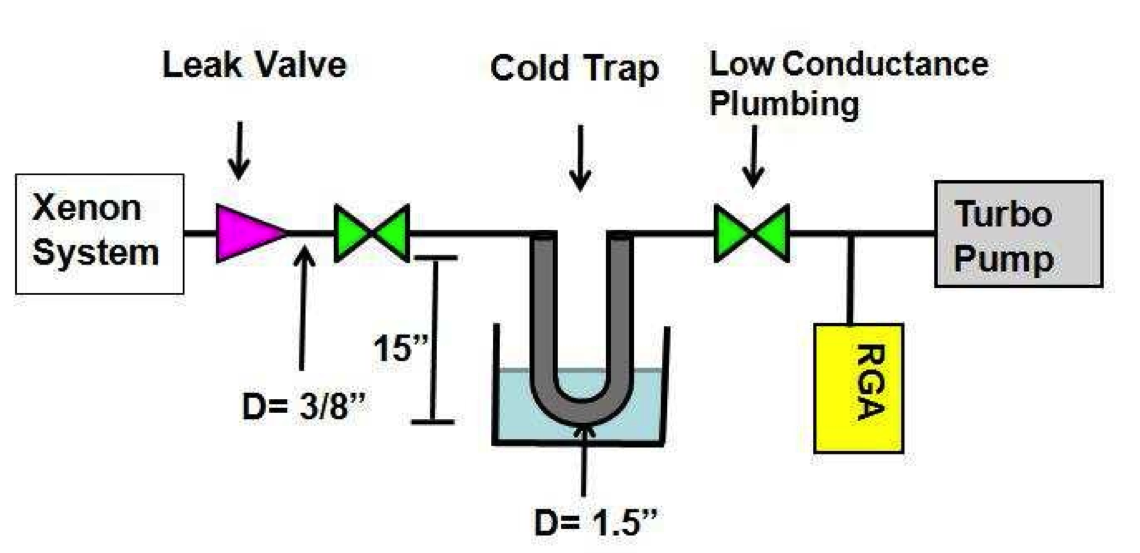
\includegraphics[width=100mm]{figures/Basic_ColdTrap.png}
\caption{Basic setup of the purity analysis technique. A coldtrap is used to remove the bulk xenon, enhancing the impurity to xenon ratio of several species of interest by up to six orders of magnitude before passing the sample to a RGA for analysis.}
\label{fig:Basic_CT}
\end{figure}

For the LUX experiment we have integrated the xenon gas analysis system into the xenon circulation panel and automated the sampling procedure using pneumatic value via slow control, the plumbing schematic is shown in Figure \ref{fig:SAM_diagram}. Xenon gas is collected from the various locations of interest along the circulation path including the input/output of the xenon gas purifier, the output of the TPC, directly from the bottle farm and the xenon storage vessel. The gas sampling is done directly from the port of interest with the lines permanently plumbed in, reducing potential for air leaks and other systematics associated with having to draw samples into bottles and shipping them elsewhere for analysis [ref]. In the case where we sample a high pressure source such as a gas cylinder or SRV (storage recovery vessel), the sampling port is located at the output of a pressure regulator. The pressure of the xenon gas sampled is set either by the regulator (for a high pressure source) or by the pressure of the LUX xenon gas system which does not exceed 3 atm absolute. In either case the sample pressure is typically between 1 and 1.5 atmospheres in the 0.80 liter sample volume (about 5 to 9 grams of xenon). A diagram showing sampling ports plumed into the LUX experiment and a schematic of the analysis system is shown in Figure \ref{fig:SAM_diagram}.

\begin{figure}[h!]\centering
%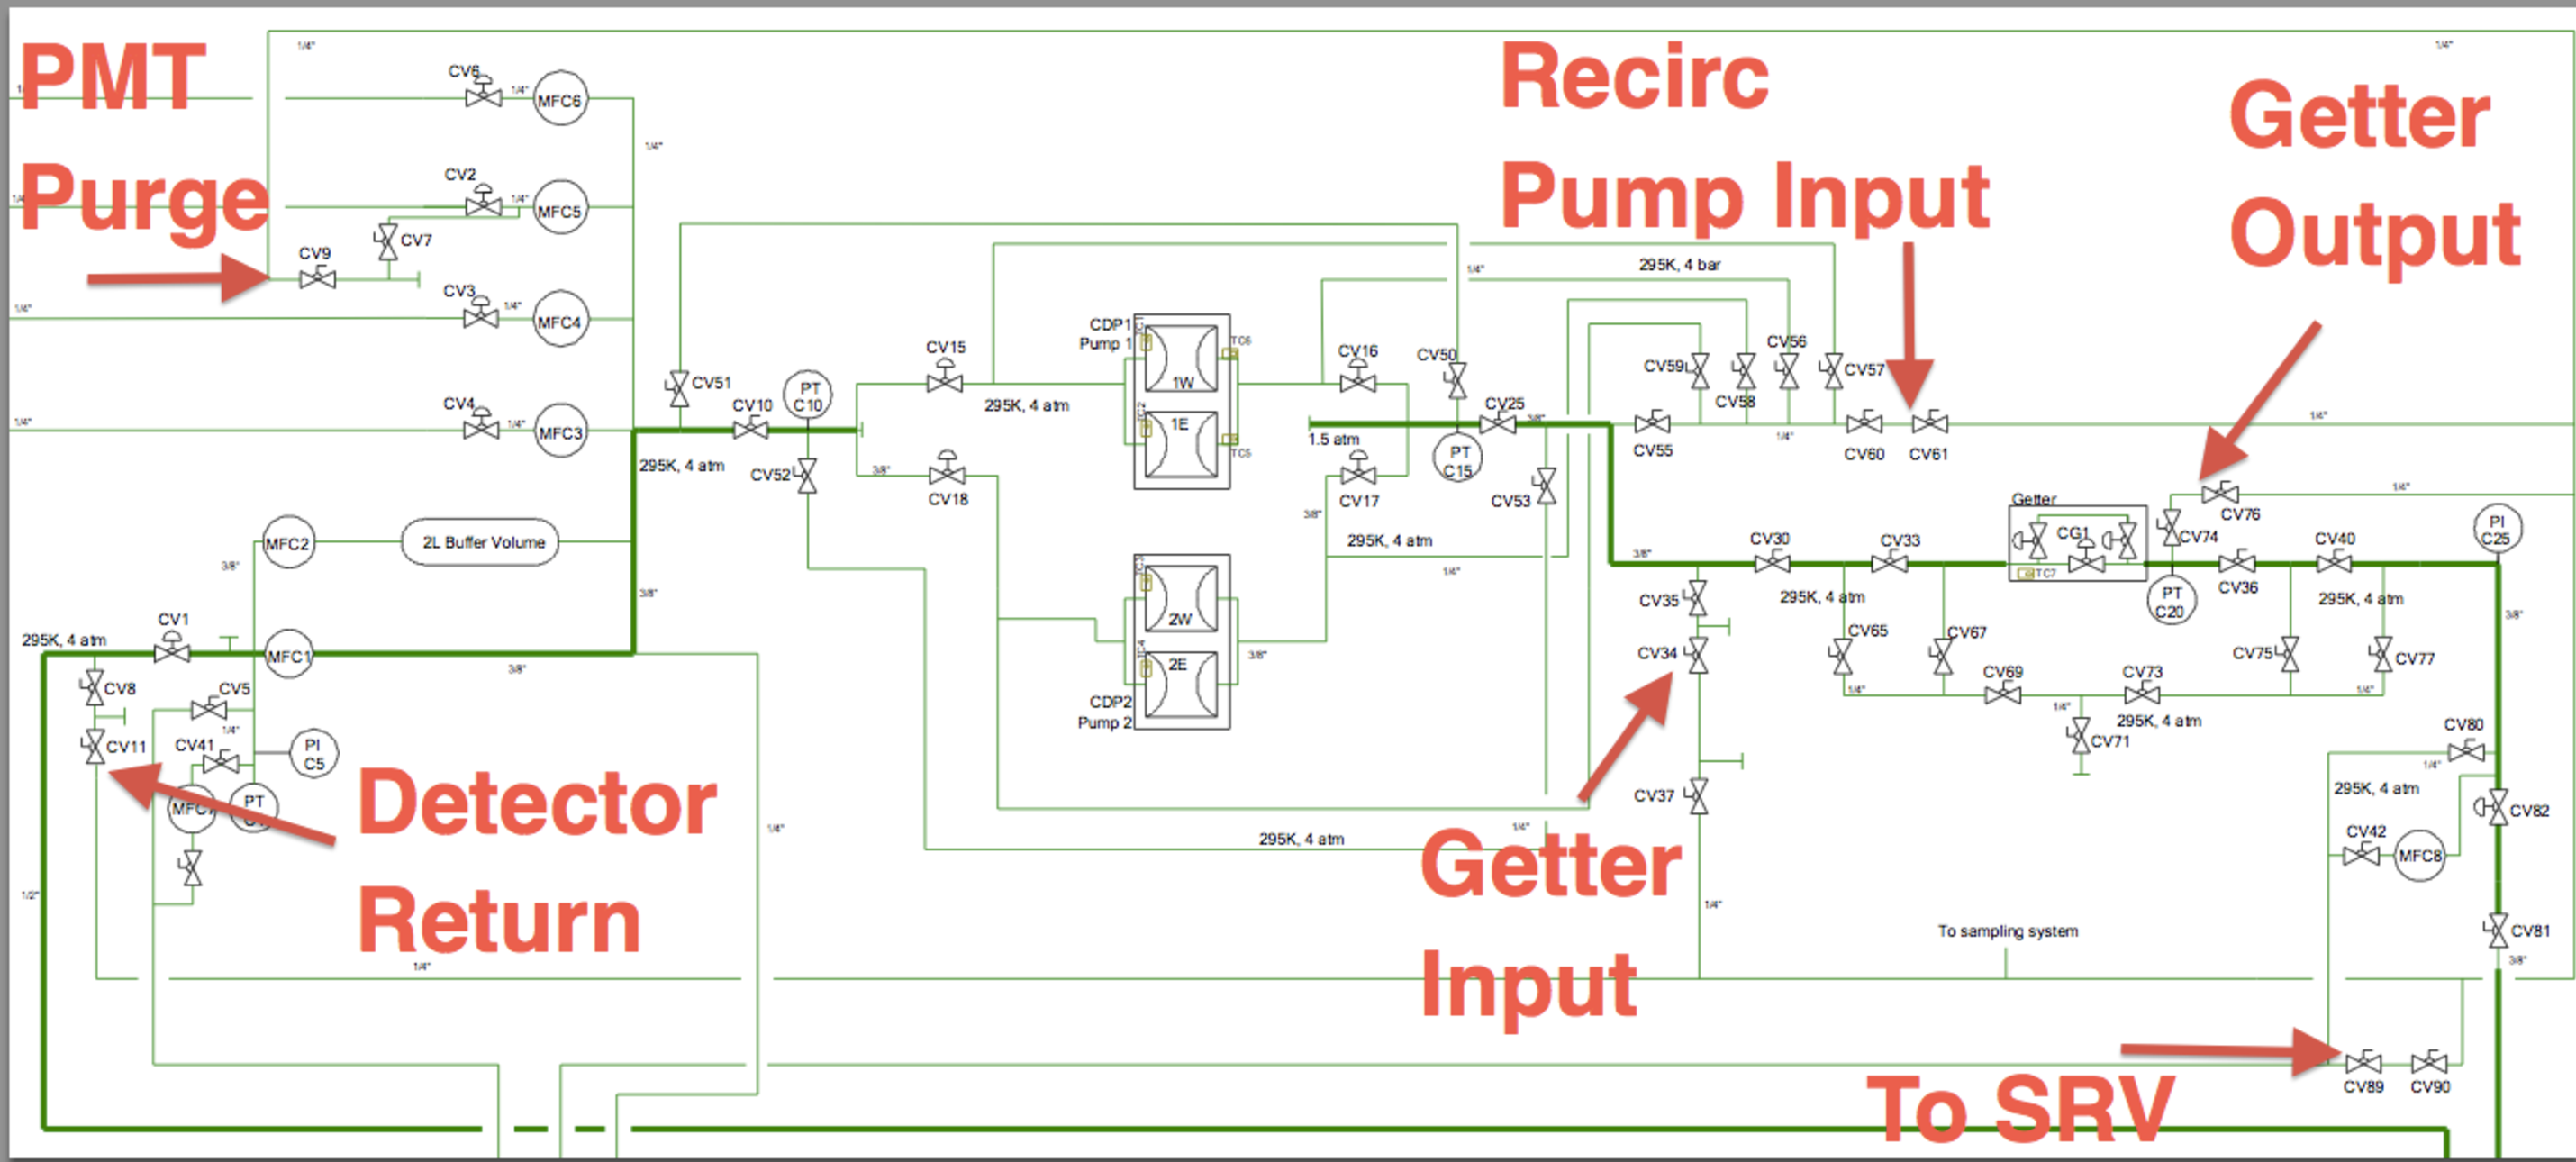
\includegraphics[width=120mm]{figures/SamplingLocations.pdf}
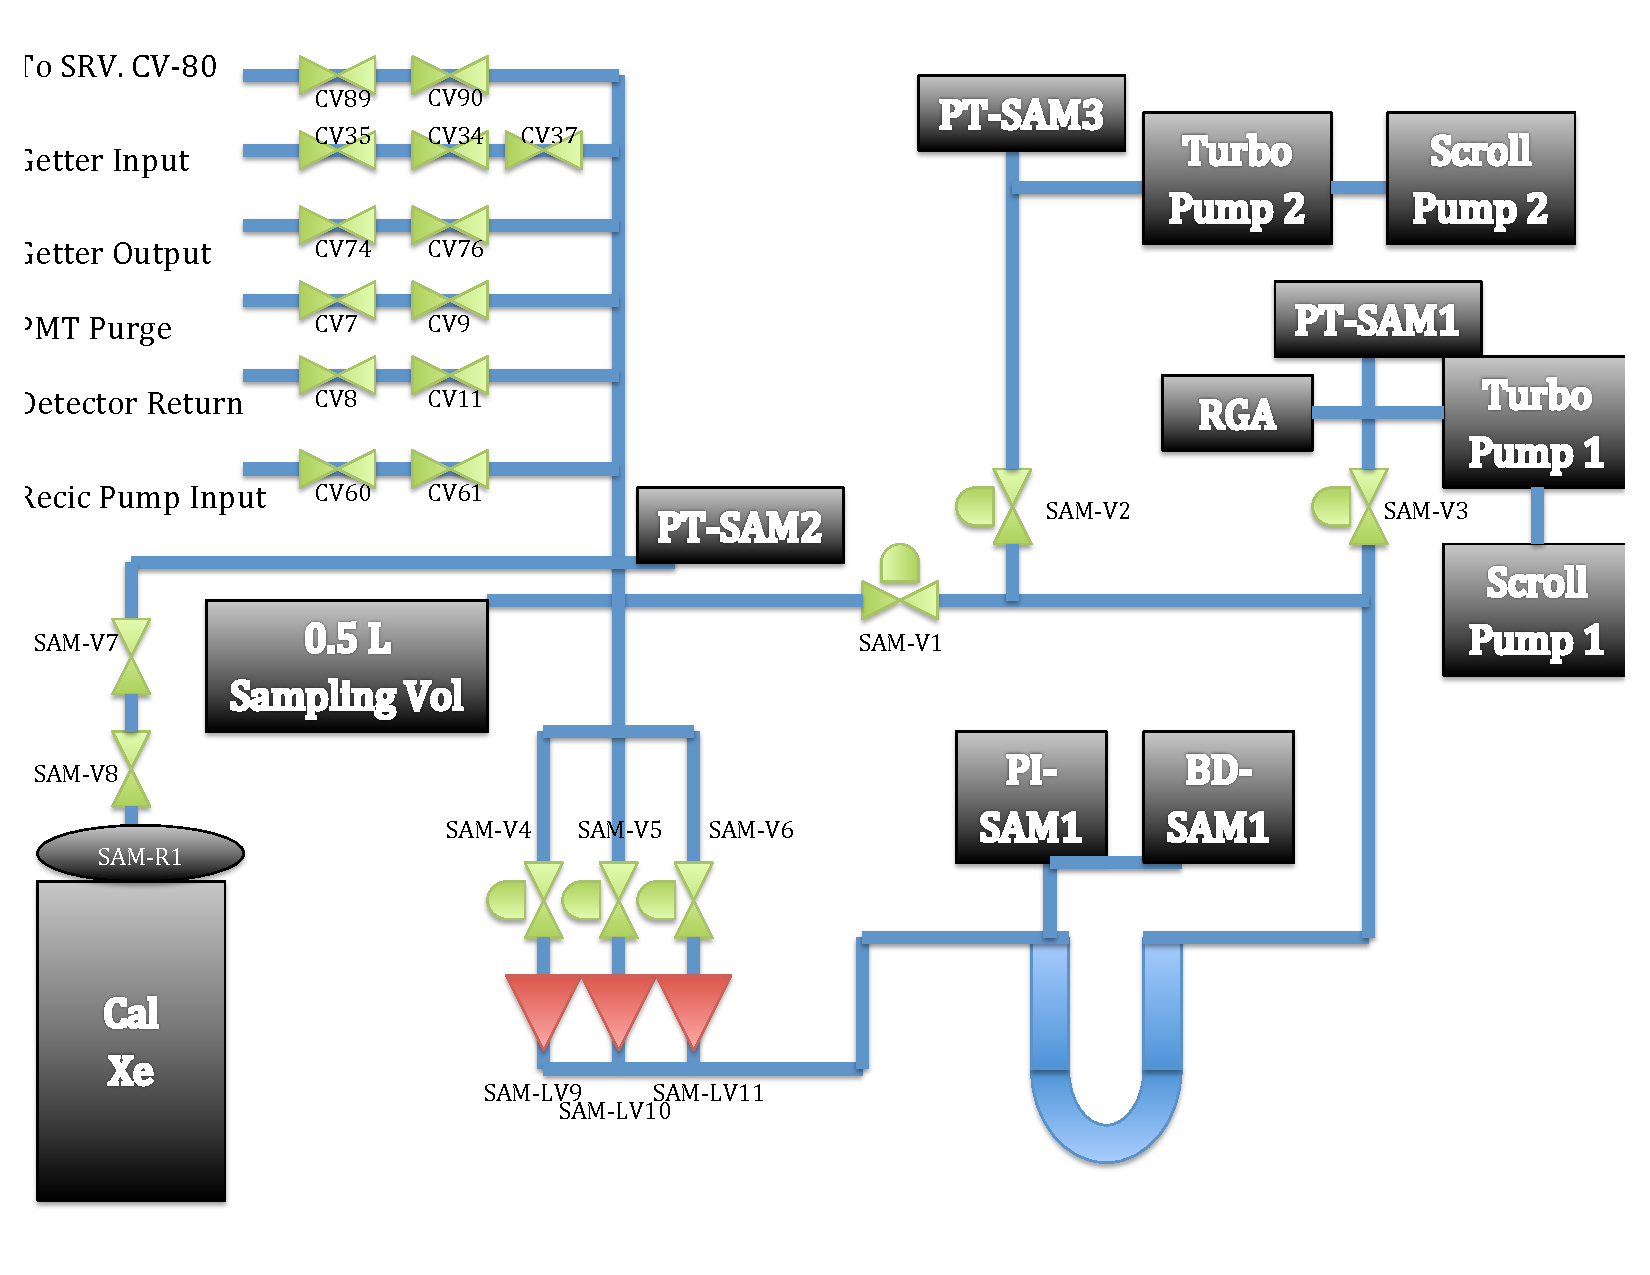
\includegraphics[width=120mm]{figures/SAM_Diagram.pdf}
\caption{A schematic of the purity analysis system, the total sampling volume is 0.80 liters. Typical sample pressures are between 1 and 1.5 atmospheres.}
\label{fig:SAM_diagram}
\end{figure}

% CCG is an order of magnitude higher than Xe because it does not include the gas type correction factor for xenon (about 0.34) and the Xe line at 132 only makes up 27\% of the natural xenon with 50% of the xenon being double ionized by the RGA and appearing at 61 amu as Xe^{++}.

% CCG gas correction factor relative to N2 and O2 for ionization vacuum gauges. H2 is about 0.5x (agrees with plot). And xenon is 2.9x
% http://www.mksinst.com/docs/UR/gaugeGasCorrection.aspx

%varian on average peff=K x indicated pressure. Xe: K=0.4. H2: K=2.4;
%http://www.idealvac.com/files/manualsII/Varian_IMG-500_Compact_Cold_Cathode_Gauge.pdf

% IMG-600 controller manual. H2: K = 2.17; Xe= K= 0.34; Ar: K= 0.77
%http://www.idealvac.com/files/ManualsII/Varian_Aglient_XGS-600_InstructionManual_2cc.pdf

%... Mention that the RGA requires < 10-5 Torr of N2 eq. to operate. Which is actually 3*10^-5 Torr Xe

The analysis system consists of a 0.5 l bottle used as a buffer volume for sampled xenon and 0.3 l of additional plumbing to the sampling ports, a capacitive manometer, three vacuum leak valves set at various leak rates, a U- shaped liquid nitrogen cold trap, a low-conductance plumbing element, an SRS RGA-200, two cold cathode vacuum gauges, two turbo pumps, two scroll pumps, six pneumatic VCR valves and instrumentation necessary for automation via a slow control interface. The capacitance manometer (MKS Baratron model 627B) measures the pressure in the sample buffer volume (0.8 l total) before and during the impurity measurement. The leak valves (part number of the ones with the dial?) admit the sampled gas to the cold trap at much reduced pressure and allows for control of the flow rate into the trap a three preset values. The cold trap consists of a U-shaped segment of 3.8 cm OD stainless steel tube with a height of 38 cm designed to be partially immersed in a liquid nitrogen bath. The low conductance element is a 10 cm segment of 0.6 cm and 0.95 cm OD plumbing with one right angle bends. A port leading to the SRV is also plumed in to the analysis system allowing for for 99.9\% of the 5 to 9 grams of sampled xenon to be recovered after the conclusion of the impurity measurement, only several milligrams of xenon are consumed for a measurements. The cold cathode gauge allows the total pressure at the RGA to be monitored and recorded. We have found it necessary to limit this pressure to less than $\rm1.0 \times 10^{-5}$ torr to prevent RGA saturation effects.
The analysis system includes a port to allow for a sample bottle filled with calibration xenon to be attached. We prepared the calibration xenon gas with known concentrations of \Otwo, \Ntwo, \He, \Ar, \Kr, and \CHfour, by mixing known quantities of these impurities with a known amount of xenon. Except where otherwise noted, all of our impurity measurements are quantified by comparing to such calibration xenon.
% Describe with Automated steps! %%-->
Once a xenon gas sample has been collected we analyze the sample for impurities as follows. The RGA is prepared to measure and record the partial pressures as a function of time of the relevant species, an RGA scan of a calibration is shown in Figure \ref{fig:RGA_Calibration}. We typically monitor, in atomic mass units, 28 (\Ntwo), 32 (\Otwo), 18 (\water), 132 (Xe), 2 ($\rm H_2$), 4 (\He), 15 (\CHfour), 40 (\Ar), and 82, 84, 86 (\Kr). We cool the cold trap with liquid nitrogen while it is still being pumped to ultra-high vacuum with the turbo pump, and then the xenon gas is admitted into the cold trap in three steps. First, the leak valve at the lowest flow setting is opened which admits xenon into the cold trap at a very small flow rate, below $10^{-4}$ standard liters per minute (SLPM). Xenon ice forms in the cold trap and the analysis system is purged of residual trace impurities by the flowing gas. We wait ten minutes for the backgrounds to stabilize before proceeding. Second, we open the leak valve to a larger flow rate, usually corresponding to an flow rate of $\sim$ 0.01 SLPM. This coarse measurement is performed to ensure that no \Ntwo from an air leak or other impurity is present at amounts that could saturate the RGA signal, if the xenon is deemed pure then the system moves on to the next higher flow stage for the 1 \ppt \Kr measurement. Third, the main leak valve is opened corresponding to flow rates of $\sim$ 0.1 SLPM gaining another factor of 10x in sensitivity from the coarse measurement. The higher flow rate used in this step allows impurities to be observed with high sensitivity, typically one part-per-billion to on part-per-trillion or better depending on the impurity species. The xenon gas in the sample bottle is slowly depleted as it flows into the cold trap. This causes the sample bottle pressure, and the flow rate through the leak valve, to decrease in time while the measurement takes place (see Figure \ref{fig:RGA_Calibration}). After a measurement period of three minutes, the leak valve is closed, the cold trap is allowed to warm to room temperature, and the xenon in the cold trap and the sample bottle is collected in the recovery bottle with liquid nitrogen. After the sample we take an RGA mass spectrum scan (1-200 amu) of the cold trap at room temperature to look for impurity species such as \water, solvents, or heavy hydrocarbons which would be trapped in the cold trap at liquid nitrogen temperature.
Note that to achieve the best sensitivity, the highest possible flow rate should be used for each measurement, limited only by RGA saturation effects. 

\begin{figure}[h!]\centering
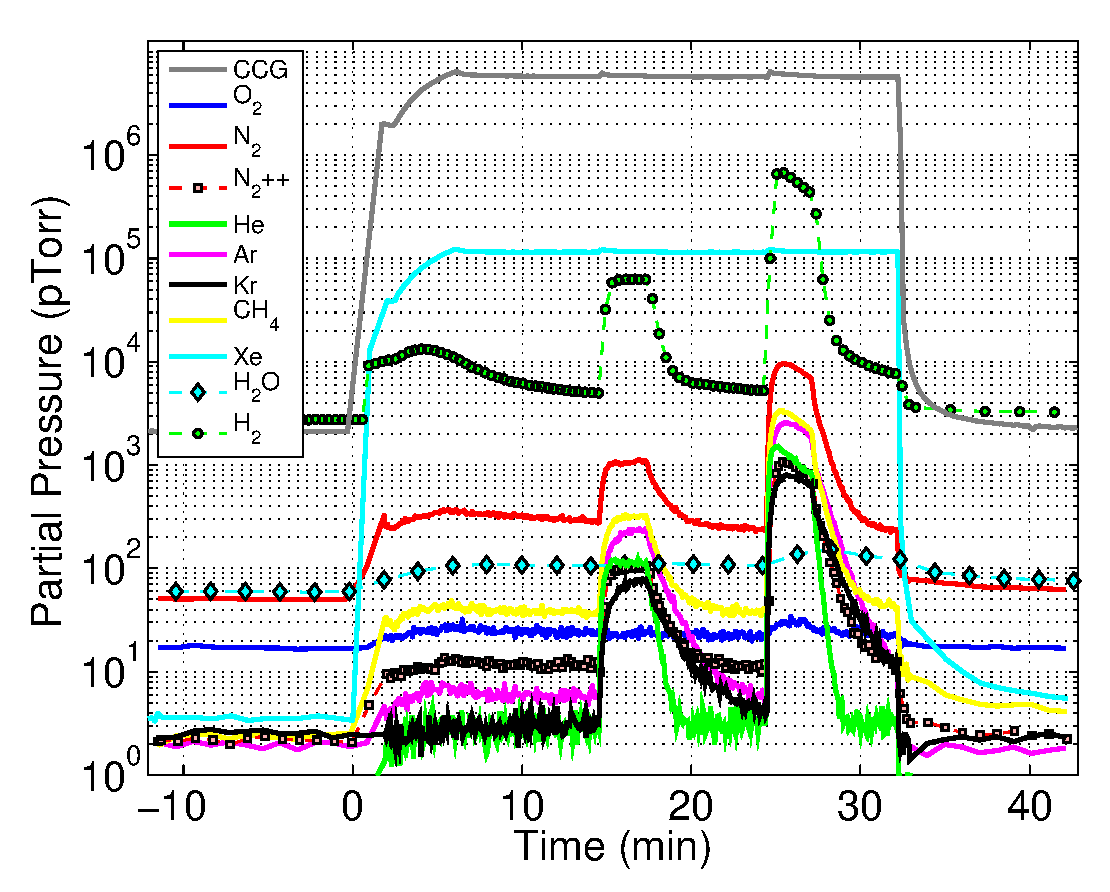
\includegraphics[width=130mm,]{figures/2013-June-05_Cal.eps}
\caption{Typical RGA calibration measurement. (CCG pressure appears higher because of a gas correction factor of 3x for xenon, 132 amu is only 1/4 of the total naturally occurring xenon and because half of xenon is double ionized appearing at 66 amu).}
\label{fig:RGA_Calibration}
\end{figure}

\section{Purity Measurement}

% 1) Know the flow rate and wait for signals to stabilize. [Coldtrap and Purifier paper].
   %2) Finite sample with declining input pressure. Use peak partial pressure normalized to flow rate [EXO and Kr paper].
   %3) ... here we integrate the signal from 30 to +180 s after the valve is opened. And divide by the average flow rate. and also normalize to Xe PP.
   
%Previous experiments have shown that the RGA partial pressures of many impurity species of interest are proportional to both their concentration in the xenon gas and to the flow rate through the leak valve[5]. After the flow is induced, the integrated partial pressures divided by the flow rate therefore gives a figure-of-merit which is proportional to the impurity concentration, and this figure-of-merit can be calibrated in terms of absolute concentration using xenon gas of known purity.

%%

For a given leak rate the measured RGA partial pressures have been found to be proportional to the impurity concentration over several orders of magnitude [ref]. In practice samples are taken at a variety of initial pressures and the RGA gain is prone to small, daily gain drifts. To account for the variation in initial sample pressure, which dictates flow rate through the pre set leak valve, the partial pressure signals are normalized to the average flow during the time that measurement is made. The reason being that the signal at a given atomic mass depends linearly on the number of impurities passing by per unit time. We have shown in pervious calibrations that the leak rate normalized RGA partial pressure is proportional to the impurity concentration of the xenon gas, both in the case of constant flow or declining flow [ref ref]. We also find for the LUX purity analysis system, that the leak rate normalized partial pressure is well behaved and is discussed further in this section. Due to power outages and environmental variables the RGA is subject to daily gain shifts. The gain can be corrected for by simply calibrating the device each time the RGA is power cycled. However, frequent calibrations may not be practical over months of running so we present a convenient method to normalize the RGA's gain by tracking xenon vapor pressure.

\subsection{RGA Partial Pressure Measurement}

A typical quadrupole mass spectrometer (such as the SRS RGA-200) measures the partial pressures of impurity species under vacuum conditions by trapping ionized particles at a given frequency for which the charge to mass ratio is in resonance. The particles are ionized by electrons released through thermionic emission from a hot filament and then accelerated through a 70-90 V potential. Due to the bombardment of electrons, atoms and diatomic molecules, such as Xe and \Ntwo, may become doubly ionized and appear at half of the expected charge to mass ratio. One the other hand, molecules such as methane and carbon monoxide can be cracked and show up at masses corresponding to a lost hydrogen or split molecule, respectively. For the measurements reported in this work we track the masses given in Table \ref{table:RGA_Species}. For a select species we report on the typical amount that a diatomic molecule or atom is doubly ionized by the RGA at 90eV in Table \ref{table:RGA_Double}. Knowing these parameters is crucial for ensuring that measurements for the expected \Ntwo signal at 28 AMU is really nitrogen and not carbon monoxide or that the expected \meth signal at 16 AMU is not contaminated by $\rm O_2^{++}$. For the case of \meth we track 15 AMU corresponding to $\rm CH_3^{+}$, which makes up a sufficient 40\% of the total methane signature without the potential for contamination at 16 amu from \Otwo or cracked \water. Xenon and Krypton, being relatively easily ionizable, show up 40\% and 20\% doubly ionized, respectively. For the most important specie of interst, Kr, we measure not only the most abundant isotope at 84 amu (57.0\%) but also the next two significant isotopes 86 amu (17.3\%) and 82 amu (11.6\%). Measuring 82+84+86 instead of simply 84 was found to boost the Kr sensitivity by exactly what was expected by counting the additional isotopes, an increase of 50\%. Additionally, using the ratios of the krypton isotopes is a powerful tool for discriminating potential hydrocarbon backgrounds from a legitimate krypton signal.  Though not implemented in this work, another 20\% gain in krypton sensitivity can be achieved by looking for the doubly ionized $\rm Kr^{84}$ signal at 42 amu and $\rm Kr^{86}$ 43 amu, doubly ionized $\rm Kr^{82}$ at 41 amu may have contamination from the argon peak at 40 amu. 

\begin{table}[h!]
%\caption{Nonlinear Model Results}
\centering
\begin{tabular}{|c| |c| |c|}
\hline
AMU & Primary Use & Secondary Use \\ [0.5ex] % inserts table %heading
\hline
2	&	$\rm H_2$			&  HydroCarbon, \water \\
4	&	\He					&								 \\ 
12	&	C					&   CO, HydroCarbon \\
14	&	$\rm N_2^{++}$ 	& 								 \\
15 & 	\meth (40\%)		& 								 \\ 
16	&	 $\rm O_2^{++}$	& \meth(45\%), \water, CO \\
18	&	\water				&								 \\
28	&	\Ntwo				& CO							 \\	
32	&	\Otwo				&								 \\
40	&	\Ar					&								 \\
44	&	$\rm CO_2$		&								 \\
82	&	\Kr (11.6\%)		&								 \\
84	&	\Kr (57.0\%)		&								 \\
86	&	\Kr (17.3 \%)		&								 \\
132&	Xe (26.9\%)		&								 \\[0.5ex]

\hline
\end{tabular}
\caption{Partial pressures of impurity species (in AMU) tracked by the RGA during the purity analysis. }
\label{table:RGA_Species}
\end{table}

\begin{table}[h!]
%\caption{Nonlinear Model Results}
\centering
\begin{tabular}{|c| |c| |c| |c|}
\hline
Species & AMU &	$\rm ^{++}$ AMU 	& $\rm ^{++}$ Fraction \\ [0.5ex] % inserts table %heading
\hline
\Ntwo	& 28			& 14	&  10\%	\\
\Otwo	& 32			& 16	&  10\%	\\ 
\Ar		& 40			& 20	&  10\%	\\
\Kr		& 84 (57.0\%)	 & 42	&  20\%	\\
Xe		&132 (26.9\%)& 66	&  40\%	\\[0.5ex]
\hline
\end{tabular}
\caption{Typical values for the fraction of doubly ionized atoms and diatomic molecules at the RGA's electron acceleration potential of 90 V.}
\label{table:RGA_Double}
\end{table}


\subsection{Correcting for RGA Gain Drift}

Before discussing calibration and purity measurements we must consider the stability of the RGA signals which can be effected by environmental variables. To our advantage there is a convenient way to monitor the gain of the RGA by tracking the one constant linking all xenon samples, the xenon vapor pressure. Since a liquid nitrogen bath is used for the impurity detection technique the dominant xenon pressure is always fixed in the coldtrap at 1.8 mtorr and 77K [ref]. The xenon vapor pressure is independently checked with a cold cathode gauge near the turbo pump, and is found to be stable within 3\% over the course of measurements from January 2013 to January 2014. Thus, any changes in the xenon RGA measurement while pumping on xenon ice (as long as the CCG and turbo pump current are fixed) is an indication of a shift in the RGA's gain. We corrected for daily changes in the RGA gain by normalizing the RGA signals to the xenon pressure of the measurement. Figure \ref{fig:RGA_Gain} shows the average xenon pressure measured by the RGA for each measurement and calibration over the corse of a year. There are variations up to a factor of ten in the RGA's response that need to be corrected for, it is not sufficient to simply use the nearest calibration point. Figure \ref{fig:RGA_Corr_Cal} shows the difference normalizing the measurement to xenon vapor pressure makes in the signal stability.

% Reference plot showing the LRN signal vs. Gain Corrected-LRN signal.

\begin{figure}[h!]\centering
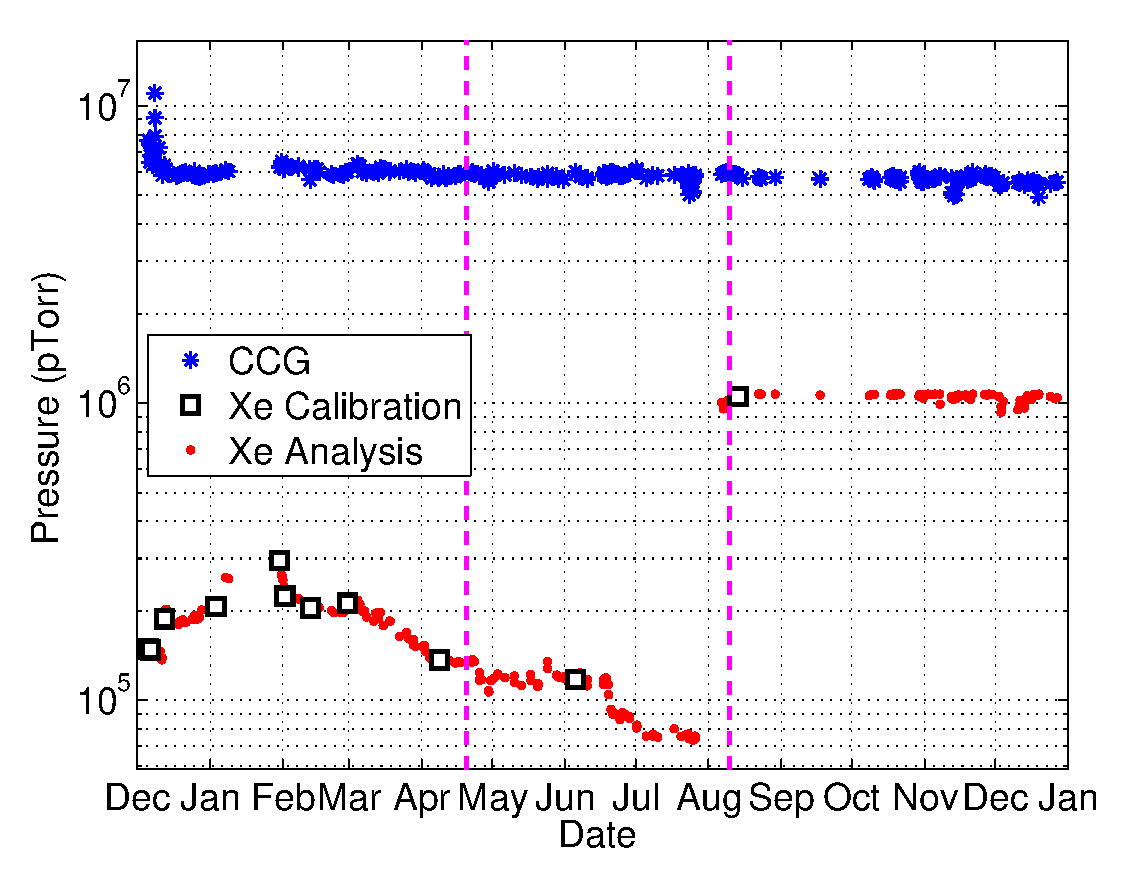
\includegraphics[width=100mm,]{figures/SAM_RGA_Gain_Run03.eps}
\caption{Xenon vapor pressure as measured by the RGA and CCG over the course of the LUX underground science run.}
\label{fig:RGA_Gain}
\end{figure}


\subsection{Correcting for Flow Rate}

The measurements described in this article differ from that of Ref. [coldtrap paper] in that only a modest quantity of xenon gas is used for analysis in each sample, typically one standard liter, note that since xenon freezes in the coldtrap the sample is entirely recovered after the analysis. The sample pressure noticeably decreases during the measurement process, and also the mean flow rate varies between subsequent samples with the initial sample pressure. We account for the varying flow rate as follows. We normalize the average integral of the RGA signal to the integral of the flow rate, the leak rate normalized RGA partial pressure has been found to be constant in previous calibration [Kr paper, EXO ref] . Therefore the integrated RGA partial pressure of the impurity, which are measured in the first three minutes of flow, also depend on the average flow rate as the number of impurities that pass by the RGA per unit time is proportional to the flow. As shown in Figure \ref{fig:RGA_Flow}, we have measured this dependence for gain corrected \Ntwo, \He, \Ar, \CHfour, and \Kr signals, at our nominal flow settings, using xenon gas from our calibration cylinder over a several month period. The data is well described by a simple linear fit for the dependence of gain corrected signal vs. mean flow rate.

\begin{figure}[h!]\centering
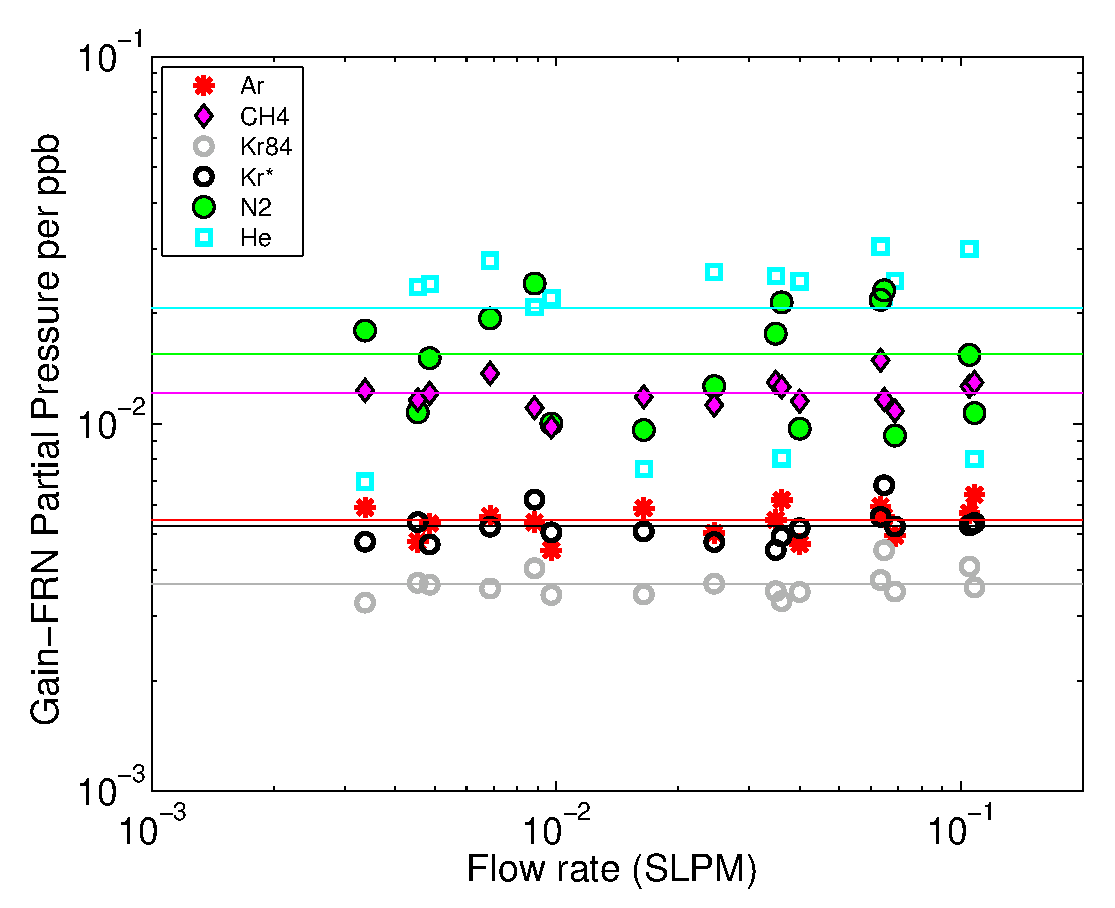
\includegraphics[width=100mm,]{figures/SAM_RGA_Cal_Run03_corr_flow.eps}
\caption{Gain corrected and leak rate normalized signals vs. flow rate for calibration xenon over eight months. The dominant source of variation is the RGA gain drift over time. (N2 and He calibration off by 2x, CH4, Ar, Kr are within 30\%).}
\label{fig:RGA_Flow}
\end{figure}

\subsection{Gain and Flow Corrected Figure of Merit}

To monitor for daily variations in the system response, including changes in the RGA gain, we periodically calibrate the analysis system using our cylinder of calibration xenon gas. After performing a periodic calibration we normalize the integral of the RGA partial pressure for a given species to both flow and the xenon partial pressure. First, the flow normalization is to remove the linear dependance of the signal on flow. Secondly, we correct for a drift in the RGA gain by normalizing to the partial pressure of \Xe which is the one true constant between all samples as it represents the xenon ice vapor pressure at 77 K in the coldtrap system (given a fixed CCG pressure). Using these normalizations we find repeatable measurements for a given impurity concentration over a range of flows and several months of RGA calibration. (will go into more detail about N2,H2 ... and the well behaved CH4, Ar, Kr).
Figure \ref{fig:RGA_Corr_Cal} shows the variations in the system response to various impurities for out calibration xenon over a period of eight months with and without the xenon vapor pressure gain correction.  

\begin{figure}[h!]\centering
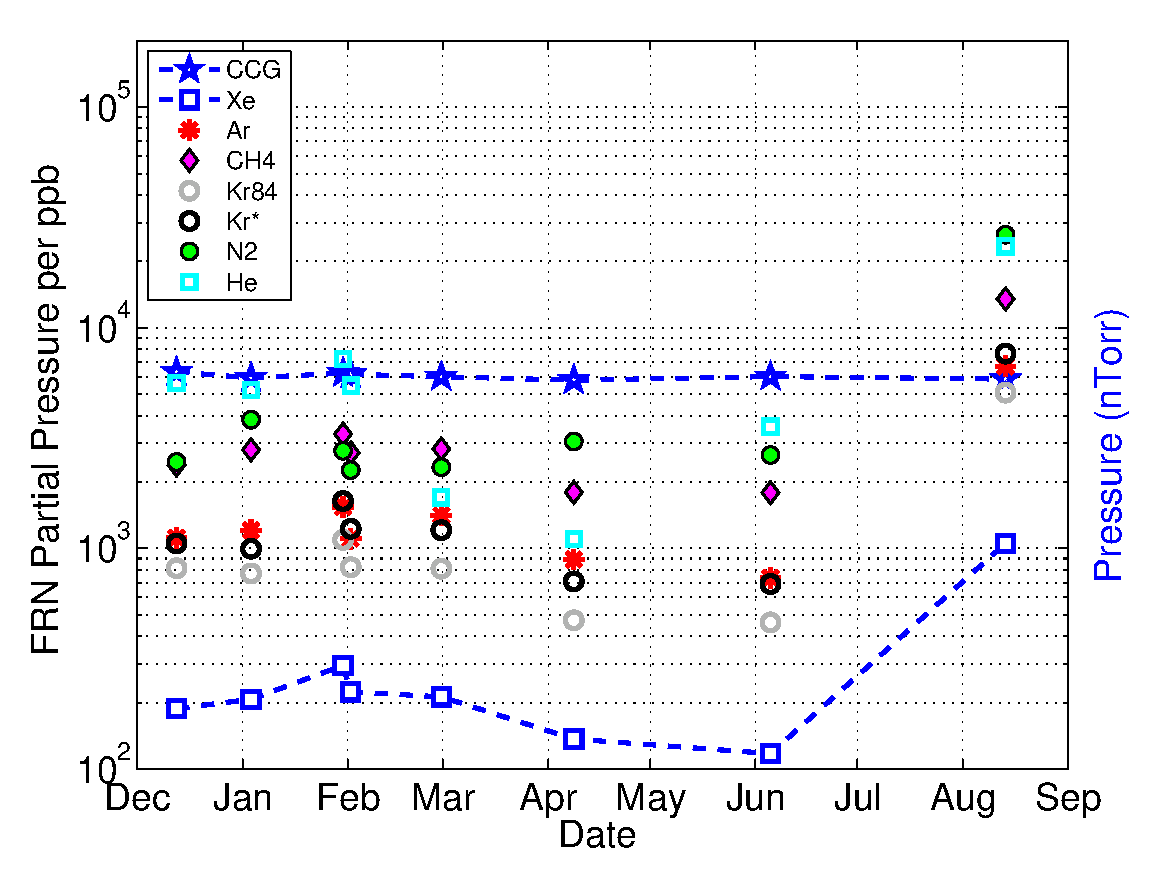
\includegraphics[width=100mm,]{figures/SAM_RGA_Cal_Run03.eps}
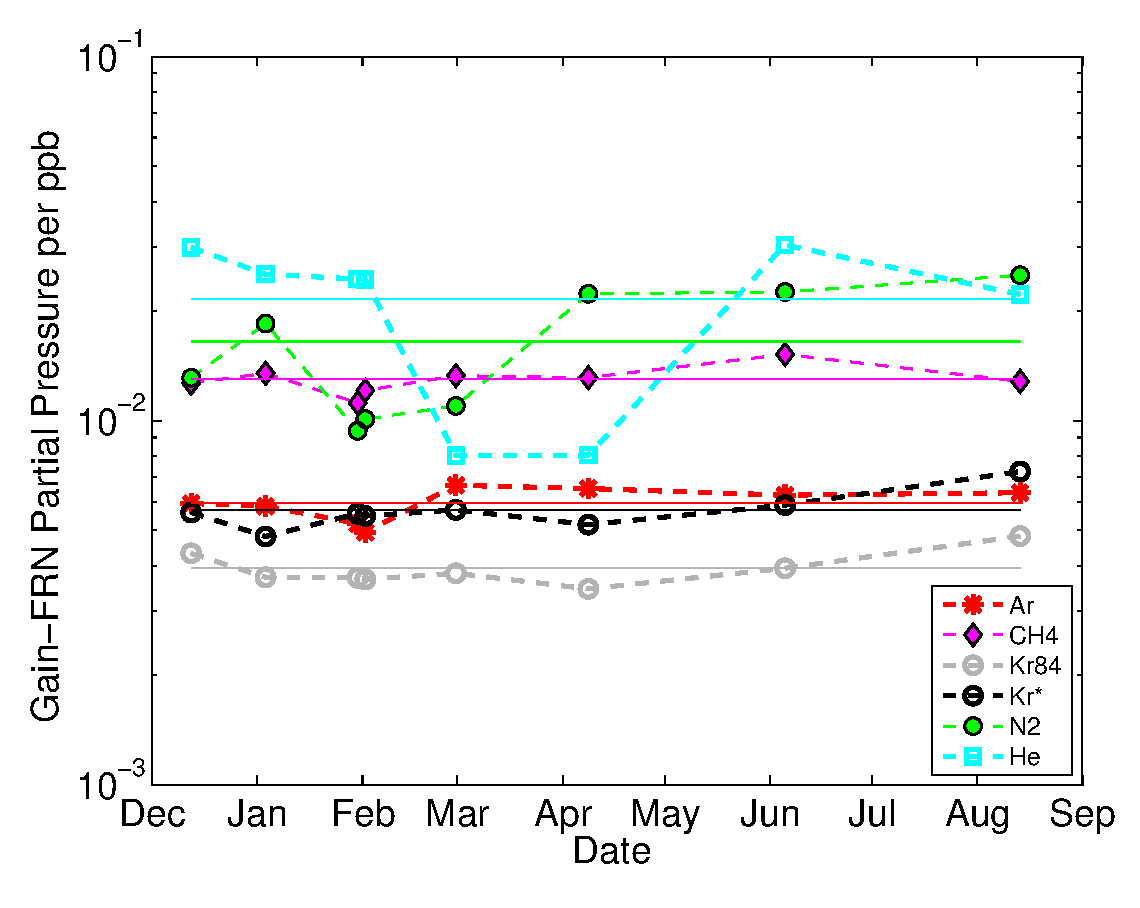
\includegraphics[width=100mm,]{figures/SAM_RGA_Cal_Run03_corr.eps}
\caption{Top: Leak rate normalized RGA signals for several calibration species over eight months, the left axis shows the xenon vapor pressure measured by the RGA and cold cathode gauge (CCG). We find a strong correlation between the xenon vapor pressure and the variations in the leak rate normalized signals for N2, CH4, Ar, Kr (Helium...). Bottom: Gain corrected and leak rate normalized signals for calibration xenon over eight months.}
\label{fig:RGA_Corr_Cal}
\end{figure}



The measurement is made as follows, a full RGA scan of a typical calibration is shown in Figure \ref{fig:RGA_Calibration} . First, before the flow is induced the backgrounds of all impurity species are averaged for 60 seconds to record the baselines. Second, a command is sent to actuate a pneumatic valve opening a path from the sampling volume through one of the three leak valves into the coldtrap and RGA (see Figure []). Once the valve feedback confirms the open state, the code waits 30 seconds to establish a stable flow and mitigate any transient effects. Third, all RGA signals and the flow rate are averaged over 150 seconds while the xenon flows from the sampling volume through the leak valve. During the measurement time about 60-70\% of the sample is consumed and as the sample pressure depletes the flow rate diminishes thus, it is not practical to drag out the sample measurement to the last drop. Finally, the pneumatic value in front of the leak valve is shut cutting off flow to the cold trap. The signals on the RGA a measured for an additional ten minutes to ensure that the initial background levels return. It is important to note that all measurement timing is controlled with pneumatic valves via a C script on a slow control computer, also the flow settings dialed in on the three leak valves are permanently fixed. These measures were taken for the LUX analysis system to help mitigate systematic uncertainties accosted with a human opening and closing the sensitive leak valves at measurement. In our early trials the flow of a given dial setting, after closing and reopening, was found to vary as much as 20\% [coldtrap ref]. 

The calibration figure of merit is defined by equation \ref{eq:Cal_FM}, it is the gain corrected leak rate normalized RGA signal per \ppb of concentration for a given impurity species. All purity measurements are also normalized to flow rate and then corrected for the gain shift by taking the ratio of xenon vapor pressure. The purity measurement is divided by the pervious calibration figure of merit and converted into a impurity concentration value in units of ppb (1\ppb), given in equation \ref{eq:Purity_FM}. We take the variation in calibration figure of merit before and after a sample for each individual impurity species as a systematic uncertainty in the measurement. This uncertainty represents systematics in gain drift, the RGA's response to xenon vapor pressure, the potential for small errors in calibration. 

\begin{equation}
\rm Cal=\left<RGA[pTorr]\right>\cdot\left<Flow[SLPM]\right>^{-1}\cdot\left<XeP[pTorr]\right>^{-1}\cdot\left<Concentration[ppb]\right>^{-1}
\label{eq:Cal_FM}
\end{equation}

\begin{equation}
\rm Cal=\left<RGA[pTorr]\right>\cdot\left<Flow[SLPM]\right>^{-1}\cdot\left<XeP[pTorr]\right>^{-1}\cdot\left<Cal[ppb/SLPM]\right>^{-1}
\label{eq:Purity_FM}
\end{equation}

%\small
%\begin{equation}
%\rm Cal_{LRN}=\left(\frac{\mathlarger{\int_{t_0}^{t_1}} \mathrm{RGA_{Pressure}}\,\mathrm{d}t}{\mathlarger{\int_{t_0}^{t_1}} \mathrm{}\,\mathrm{d}t}\right)
%\mathlarger\times\left(\frac{\mathlarger{\int_{t_0}^{t_1}} \mathrm{Flow}\,\mathrm{d}t}{\mathlarger{\int_{t_0}^{t_1}} \mathrm{}\,\mathrm{d}t}\right)^{-1}
%\mathlarger\times\left(\frac{\mathlarger{\int_{t_0}^{t_1}} \mathrm{Xe_{Pressure}}\,\mathrm{d}t}{\mathlarger{\int_{t_0}^{t_1}} \mathrm{}\,\mathrm{d}t}\right)^{-1}
%\label{eq:Cal_FM}
%\end{equation}
%\normalsize

% Add a table showing mean figure of merit per ppb, and stability over 1 year Gain-LRN


%After calibrating all purity measurements are normalized to flow rate and and compared to the pervious leak rate normalized calibration. The signal is then corrected for the gain shift by taking the ratio of xenon vapor pressure during the calibration and the analysis. After correcting for flow rate and RGA gain the remaining signal is simply proportional to the purity concentration of the xenon gas sample.
%To account for these variations, we normalize the signal to the corresponding xenon vapor pressure, and we take the the deviation from the xenon vapor pressure in calibration measurements to be a systematic uncertainty. For most of our measurements, this is the dominating uncertainty in the impurity concentration measurement.

%Secondly, to account for the species-dependent response of the analysis system, including factors such as the probability that each impurity survives the cold trap and its ionization potential at the RGA filament, we apply a relative species response factor as listed in Table 1. These species response factors were empirically determined by comparing each species to O2 in separate bench test measurements at constant input pressure, and are valid to within 30\%.


% \begin{figure}[h!]\centering
%\includegraphics[width=77mm]{LY_180_Tritium_Dec_2013_Light_Yield}
%\caption{}
%\label{fig:L_Q_Yield_180_un}
%\end{figure}



\bibliographystyle{thesisbibstyle}
\bibliography{TritiumBib}



\end{document}
